\section{Fake Rate Fits}
The $B^\pm$ candidates consists of the combinatorial background which spans across the fit mass range. The origin of this background type is mostly due to $J/\psi\rightarrow\mu^+\mu^-$ decays associated with random tracks. Another source of background is the Partially Reconstructed Decays (PRD) from $B$ hadron decays in which the missing four momentum impacts the final reconstruction. The unbinned extended maximum likelihood fit uses: 

\begin{itemize}
\item A Chebychev function $f(x) = 1 + \tau \cdot x$ to express the combinatorial background.
\item An error function $f(x = 1 - \text{Err}f[a_1(x-x_0)]$ to parameterize the PRD component.
\end{itemize}

A Johnson SU function has been used to parametrize the signal component. 
\subsection{Kaon - Data Fits}
\label{subsec:Fake_Rates_Fits_Kaon}

\begin{figure}[H] % <-- Use [H] here
  \centering
  \begin{minipage}[t]{0.48\textwidth}
    \centering
    \foreach \pt in {3,2,1}{
      \begin{subfigure}%{0.95\textwidth}
        \includegraphics[width=0.9\textwidth]{figures/FakeRatesFit/FakeRates/B_mass_Kaon_pT\pt_eta1}
        \caption*{$p_T=\pt$, $\eta=1$}
      \end{subfigure}
    }
  \end{minipage}
  \hfill
  \begin{minipage}[t]{0.48\textwidth}
    \centering
    \foreach \pt in {3,2,1}{
      \begin{subfigure}%{0.95\textwidth}
        \includegraphics[width=0.9\textwidth]{figures/FakeRatesFit/FakeRates/B_mass_Kaon_pT\pt_eta2}
        \caption*{$p_T=\pt$, $\eta=2$}
      \end{subfigure}
    }
  \end{minipage}
  \caption{Mass fit to the reconstructed $B$-mass to extract the yield of $N_{K^\pm}$ from data on the different $p_{\text{T}}$ and $\eta$ bins. }
\end{figure}
\newpage

\subsection{Faking $K^\pm\to\mu^\pm$ - Data Fits}
\label{subsec:Fake_Rates_Fits_Kaon_Muon}
\subsubsection{Loose Working Point}
\begin{figure}[H] % <-- Use [H] here
  \centering
  \begin{minipage}[t]{0.48\textwidth}
    \centering
    \foreach \pt in {3,2,1}{
      \begin{subfigure}%{0.95\textwidth}
        \includegraphics[width=0.9\textwidth]{figures/FakeRatesFit/FakeRates/B_mass_Muon_pT\pt_eta1_loose}
        \caption*{$p_T=\pt$, $\eta=1$}
      \end{subfigure}
    }
  \end{minipage}
  \hfill
  \begin{minipage}[t]{0.48\textwidth}
    \centering
    \foreach \pt in {3,2,1}{
      \begin{subfigure}%{0.95\textwidth}
        \includegraphics[width=0.9\textwidth]{figures/FakeRatesFit/FakeRates/B_mass_Muon_pT\pt_eta2_loose}
        \caption*{$p_T=\pt$, $\eta=2$}
      \end{subfigure}
    }
  \end{minipage}
  \caption{Mass fit to the reconstructed $B$-mass to extract the yield of faking $N_{K^\pm\to\mu^\pm}$ from data on the different $p_{\text{T}}$ and $\eta$ bins for the Loose working point. }
\end{figure}
\newpage

\subsubsection{Tight Working Point}
\begin{figure}[H] % <-- Use [H] here
  \centering
  \begin{minipage}[t]{0.48\textwidth}
    \centering
    \foreach \pt in {3,2,1}{
      \begin{subfigure}%{0.95\textwidth}
        \includegraphics[width=0.9\textwidth]{figures/FakeRatesFit/FakeRates/B_mass_Muon_pT\pt_eta1_tight}
        \caption*{$p_T=\pt$, $\eta=1$}
      \end{subfigure}
    }
  \end{minipage}
  \hfill
  \begin{minipage}[t]{0.48\textwidth}
    \centering
    \foreach \pt in {3,2,1}{
      \begin{subfigure}%{0.95\textwidth}
        \includegraphics[width=0.9\textwidth]{figures/FakeRatesFit/FakeRates/B_mass_Muon_pT\pt_eta2_tight}
        \caption*{$p_T=\pt$, $\eta=2$}
      \end{subfigure}
    }
  \end{minipage}
  \caption{Mass fit to the reconstructed $B$-mass to extract the yield of faking $N_{K^\pm\to\mu^\pm}$ from data on the different $p_{\text{T}}$ and $\eta$ bins for the Tight working point. }
\end{figure}
\newpage

\subsection{$\pi$ - MC Fits}
\label{subsec:Fake_Rates_Fits_Pion}
\begin{figure}[H] % <-- Use [H] here
  \centering
  \begin{minipage}[t]{0.48\textwidth}
    \centering
    \foreach \pt in {3,2,1}{
      \begin{subfigure}%{0.95\textwidth}
        \includegraphics[width=0.9\textwidth]{figures/FakeRatesFit/FakeRatesPions/B_mass_Pion_pT\pt_eta1}
        \caption*{$p_T=\pt$, $\eta=1$}
      \end{subfigure}
    }
  \end{minipage}
  \hfill
  \begin{minipage}[t]{0.48\textwidth}
    \centering
    \foreach \pt in {3,2,1}{
      \begin{subfigure}%{0.95\textwidth}
        \includegraphics[width=0.9\textwidth]{figures/FakeRatesFit/FakeRatesPions/B_mass_Pion_pT\pt_eta2}
        \caption*{$p_T=\pt$, $\eta=2$}
      \end{subfigure}
    }
  \end{minipage}
  \caption{Mass fit to the reconstructed $B$-mass to extract the yield of $N_{\pi^\pm}$ from MC on the different $p_{\text{T}}$ and $\eta$ bins. }
\end{figure}
\newpage

\subsection{Faking $\pi\pm\to\mu^\pm$ - MC Fits}
\label{subsec:Fake_Rates_Fits_Pion_Muon}
\subsubsection{Loose Working Point}
\begin{figure}[H] % <-- Use [H] here
  \centering
  \begin{minipage}[t]{0.48\textwidth}
    \centering
    \foreach \pt in {3,2,1}{
      \begin{subfigure}%{0.95\textwidth}
        \includegraphics[width=0.9\textwidth]{figures/FakeRatesFit/FakeRatesPions/B_mass_Muon_pT\pt_eta1_loose}
        \caption*{$p_T=\pt$, $\eta=1$}
      \end{subfigure}
    }
  \end{minipage}
  \hfill
  \begin{minipage}[t]{0.48\textwidth}
    \centering
    \foreach \pt in {3,2,1}{
      \begin{subfigure}%{0.95\textwidth}
        \includegraphics[width=0.9\textwidth]{figures/FakeRatesFit/FakeRatesPions/B_mass_Muon_pT\pt_eta2_loose}
        \caption*{$p_T=\pt$, $\eta=2$}
      \end{subfigure}
    }
  \end{minipage}
  \caption{Mass fit to the reconstructed $B$-mass to extract the yield of faking $N_{\pi^\pm\to\mu^\pm}$ from MC on the different $p_{\text{T}}$ and $\eta$ bins for the Loose working point. }
\end{figure}
\newpage


\subsubsection{Tight Working Point}
\begin{figure}[H] % <-- Use [H] here
  \centering
  \begin{minipage}[t]{0.48\textwidth}
    \centering
    \foreach \pt in {3,2,1}{
      \begin{subfigure}%{0.95\textwidth}
        \includegraphics[width=0.9\textwidth]{figures/FakeRatesFit/FakeRatesPions/B_mass_Muon_pT\pt_eta1_tight}
        \caption*{$p_T=\pt$, $\eta=1$}
      \end{subfigure}
    }
  \end{minipage}
  \hfill
  \begin{minipage}[t]{0.48\textwidth}
    \centering
    \foreach \pt in {3,2,1}{
      \begin{subfigure}%{0.95\textwidth}
        \includegraphics[width=0.9\textwidth]{figures/FakeRatesFit/FakeRatesPions/B_mass_Muon_pT\pt_eta2_tight}
        \caption*{$p_T=\pt$, $\eta=2$}
      \end{subfigure}
    }
  \end{minipage}
  \caption{Mass fit to the reconstructed $B$-mass to extract the yield of faking $N_{\pi^\pm\to\mu^\pm}$ from MC on the different $p_{\text{T}}$ and $\eta$ bins for the Loose working point. }
\end{figure}
\newpage

\subsection{Fake Rates in Tight Working}
\label{subsec:Fake_Rates_Pion_TW}
\begin{figure}[!ht]
    \centering 
    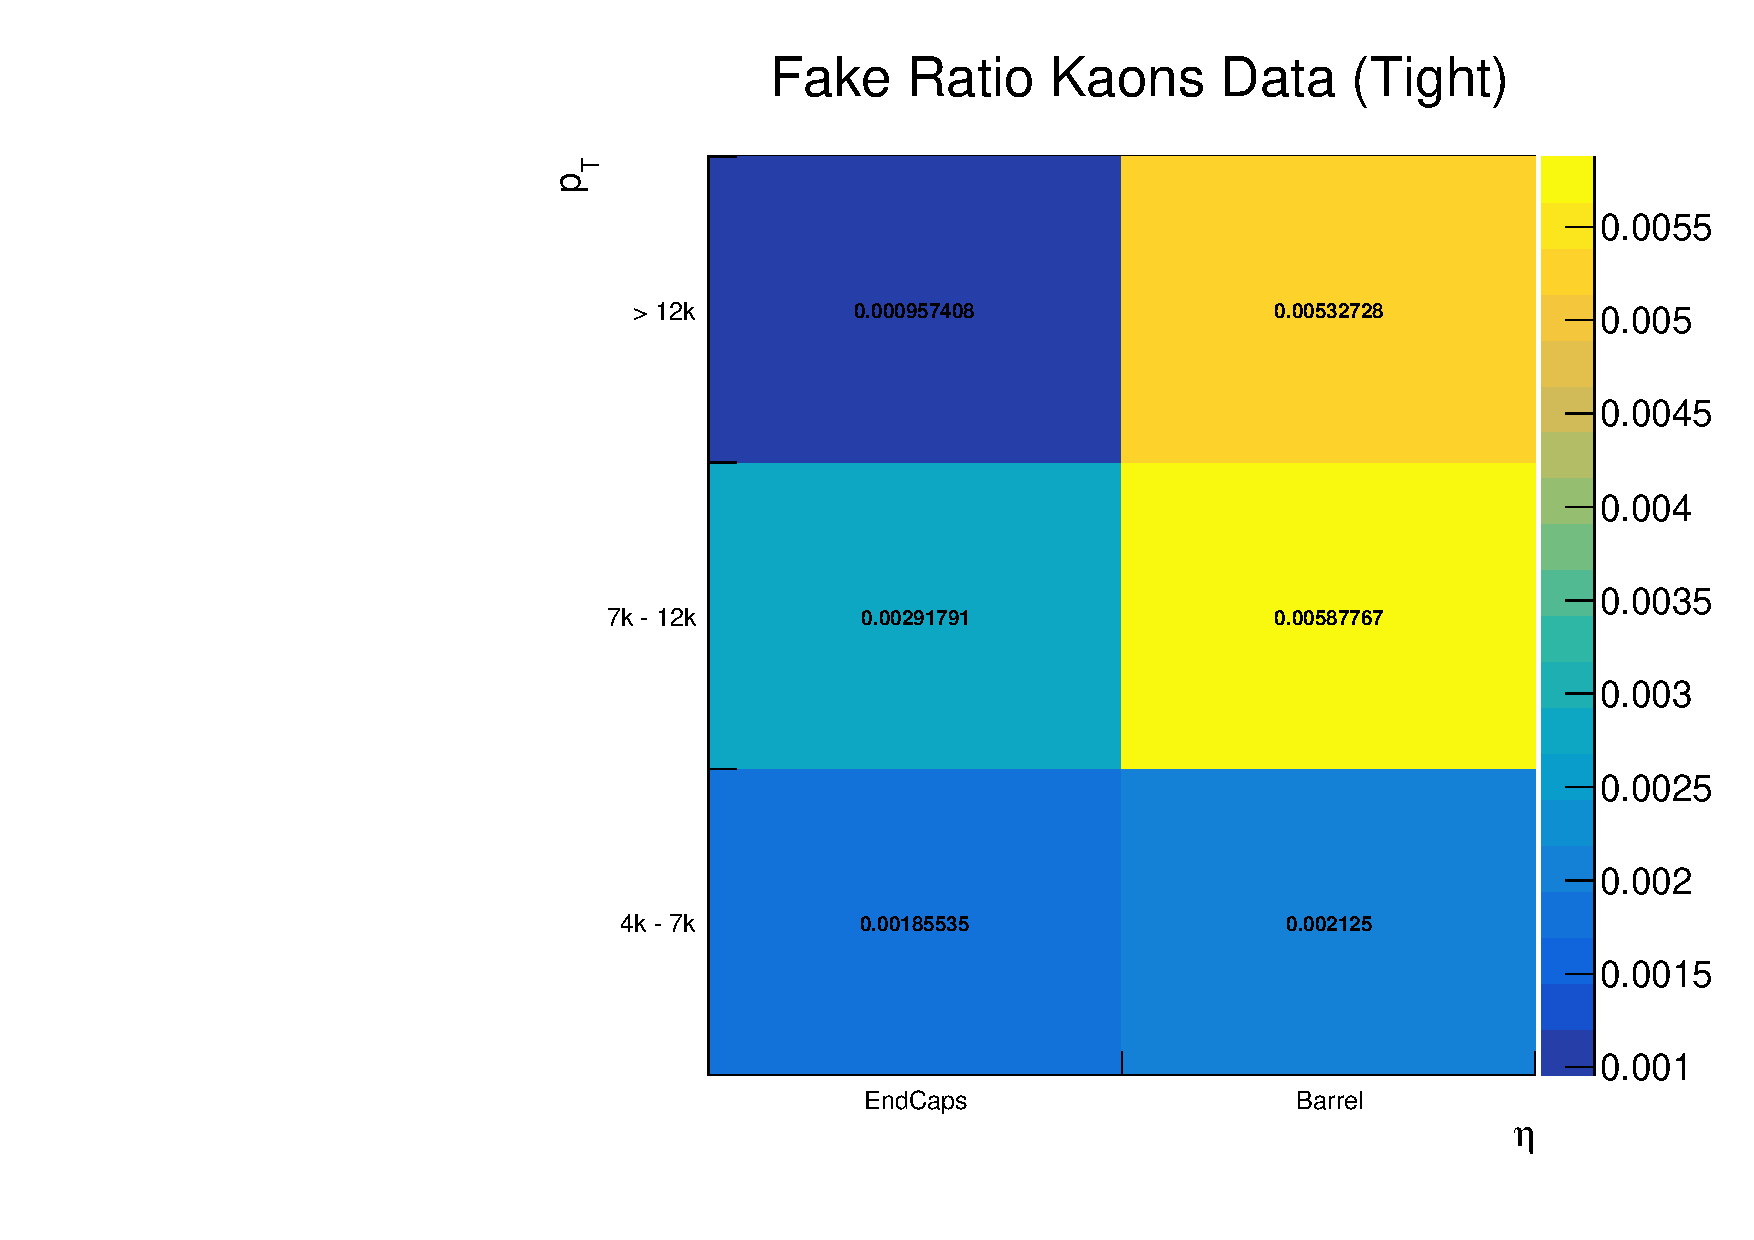
\includegraphics[width=0.45\textwidth]{figures/FakeRatesFit/FakeRates/FakeRatesTight.pdf}
    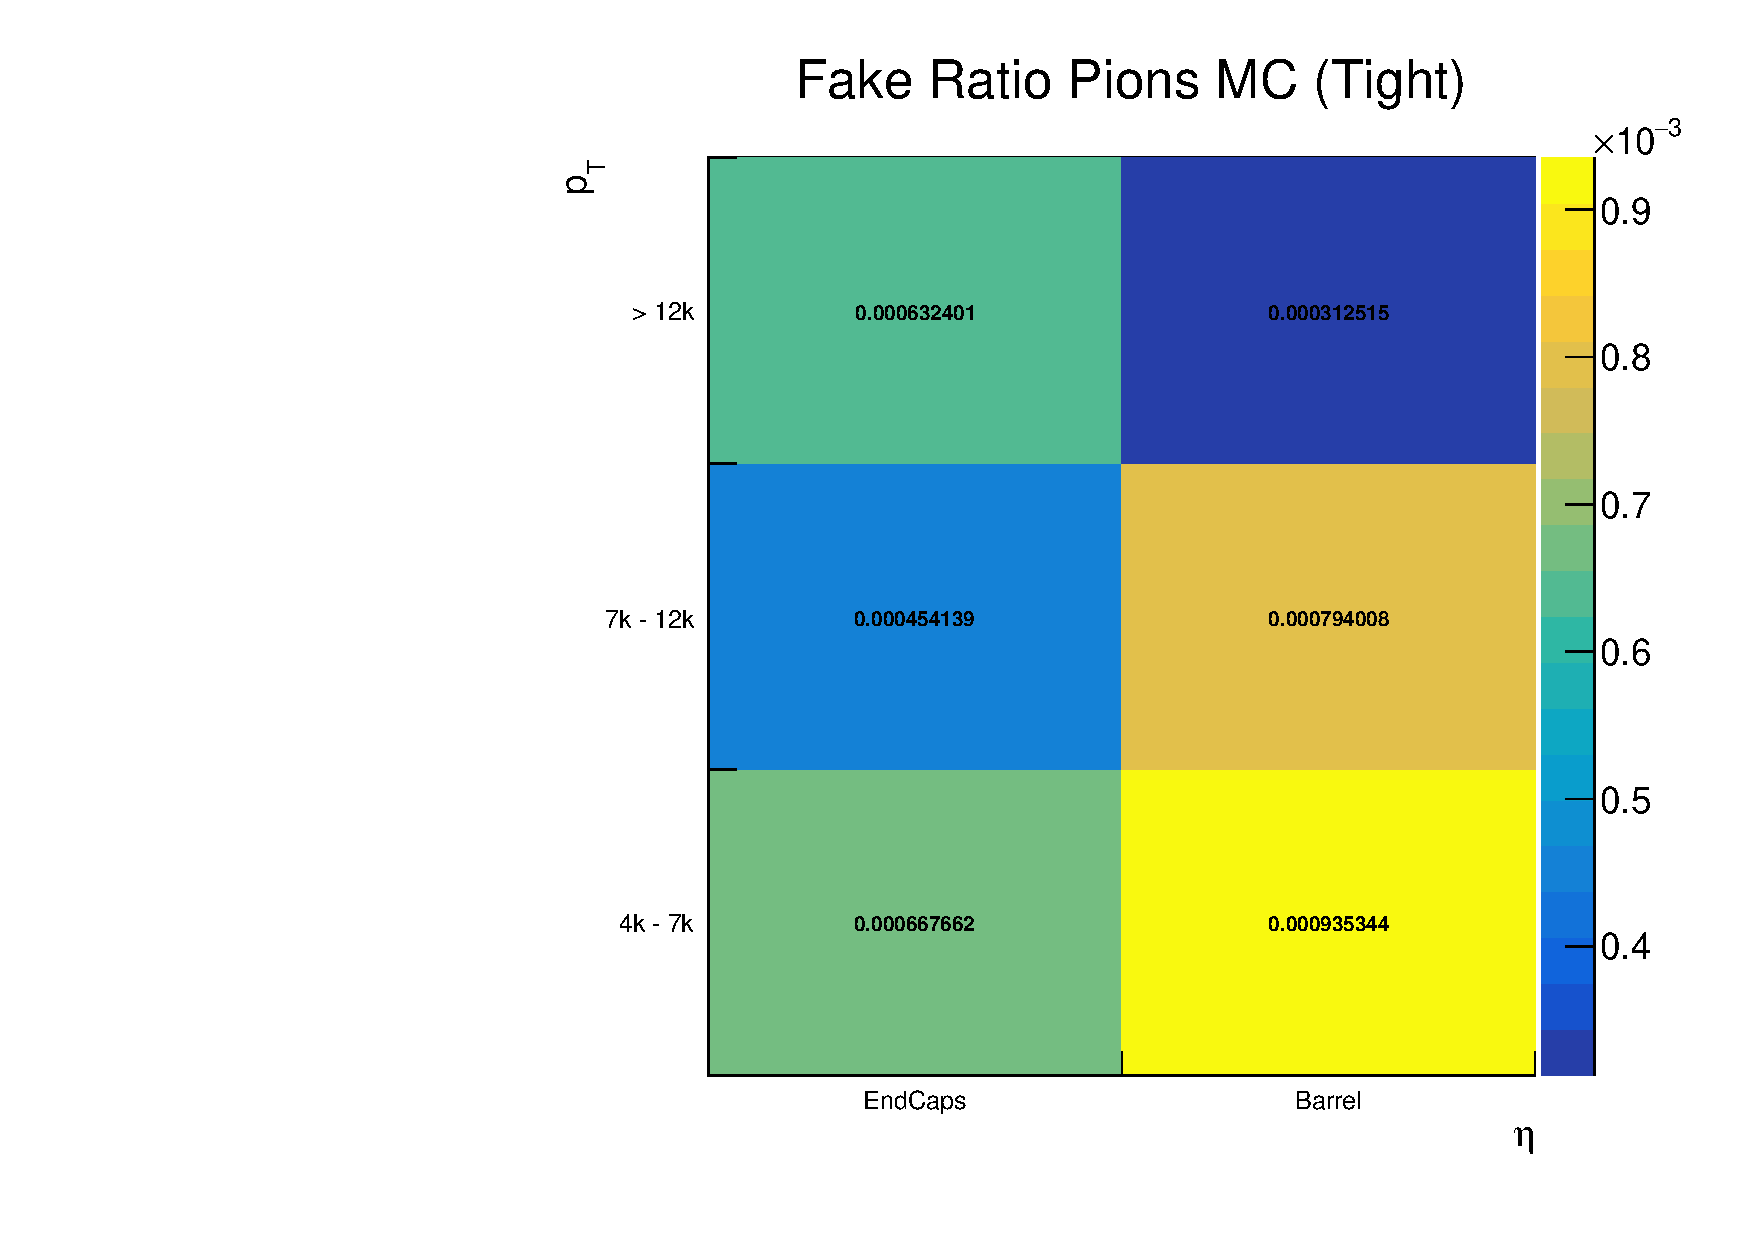
\includegraphics[width=0.45\textwidth]{figures/FakeRatesFit/FakeRatesPions/FakeRatesPionsTight.pdf}
    \caption{ Fake Rates for $P(K^\pm \to \mu^\pm)$ (left) and $P(\pi^\pm \to \mu^\pm)$ (right) in Barrel and Endcap.}
    \label{fig:K-to-ell-faking-probabilities}
\end{figure}